\documentclass{book}
\usepackage{graphicx} % Required for inserting images
\usepackage[a4paper, total={6in, 10in}]{geometry}
\usepackage[acronym]{glossaries}
\usepackage{standalone}
\usepackage{hyperref}

%needed to make table from a paper compile in LaTeX
\usepackage{booktabs}
\usepackage{makecell}
\newcommand{\emoji}[2][1.2em]{\raisebox{-0.2\height}{\includegraphics[height=#1]{#2}}}

\usepackage[style=authoryear]{biblatex}
\addbibresource{references.bib}

\title{PhD thesis on the usage on of AI models in cybersecurity education}
\author{Harry James Hall}
\date{March 2025 - ongoing}

\newacronym{llm}{LLM}{Large Language Model}
\newacronym{ai}{AI}{Artficial Intelligence}
\newacronym{dl}{DL}{Deep Learning}
\newacronym{cot}{CoT}{Chain of Thought}
\newacronym{lora}{LoRA}{Low Rank Adapter}
\newacronym{qlora}{QLoRA}{Quantized Low Rank Adapter}
\newacronym{gpt}{GPT}{Generative Pretrained Transformer}
\newacronym{llama}{LLaMA}{Large Language Model Meta AI}
\newacronym{moe}{MoE}{Mixture of Experts}
\newacronym{rnn}{RNN}{Recurrent Neural Network}
\newacronym{lstm}{LSTM}{Long Short Term Memory}
\newacronym{mha}{MHA}{Multi-Head Attention}
\newacronym{mla}{MLA}{Multi-Head Latent Attention}
\newacronym{gqa}{GQA}{Group Query Attention}
\newacronym{cuda}{CUDA}{Compute Unified Device Architecture}
\newacronym{opencl}{OpenCL}{Open Compute Library}
\newacronym{llada}{LLaDA}{Large Language Diffusion with Masking}
\newacronym{rag}{RAG}{Retrival Augemented Generation}
\newacronym{ann}{ANN}{Artificial Neural Network}
\newacronym{alice}{ALICE}{Artificial Linguistic Internet Computer Entity}

\newacronym{CPU}{CPU}{Central Processing Unit}
\newacronym{GPU}{GPU}{Graphics Processing Unit}
\newacronym{GPGPU}{GPGPU}{General-purpose computing on graphics processing units}
\newacronym{NPU}{NPU}{Neural Processing Unit}
\newacronym{RAM}{RAM}{Random Access Memory}
\newacronym{VRAM}{VRAM}{Video Random Access Memory}
\newacronym{HBM}{HBM}{High Bandwidth Memory}
\newacronym{api}{API}{Application Programming Interface}

\newacronym{ctf}{CTF}{Capture The Flag}
\newacronym{koth}{KoTH}{King of The Hill}
\newacronym{VM}{VM}{Virtual Machine}
\newacronym{irc}{IRC}{Internet Relay Chat}
\newacronym{dep}{DEP}{Data Execution Prevention}
\newacronym{aslr}{ASLR}{Address Space Layout Randomisation}
\newacronym{rop}{ROP}{Return Oriented Programming}
\makeglossaries

\begin{document}

\frontmatter

\maketitle
\tableofcontents
\chapter{Introduction}

\paragraph{}This thesis will cover the uses of \acrfull{ai} and \acrfull{dl} models such as \acrfull{llm} in educational cybersecurity simulations including hacking challenges such as \acrfull{ctf} and \acrfull{koth}. This will include using \acrshort{llm}(s) to generate narrative content (backstory), provide realistic personas for students to interact with, and even generate randomized challenges such as unique malware for malware analysis challenges.

\paragraph{}Modern \acrshort{llm}s are typically made up of transformer variants such as \acrfull{gpt}. These replaced older language model types such as \acrfull{lstm} models which are a type of \acrfull{rnn}. Transformer models were introduced in the paper \textcite{vaswani_attention_2023} by engineers at Google. These had better scalability and performance than the existing \acrlong{rnn} based approaches. One of the key features of transformers is the \acrfull{mha} mechanism. In some newer models this has evolved into techniques such as \acrfull{mla} and \acrfull{gqa} which are less computationally intensive. This thesis will be mainly looking at these transfomer based \acrshort{llm}s, though other kinds of \acrshort{llm}s such as \acrfull{llada} based models could be used. \acrshort{llada} is a novel kind of \acrshort{llm} which makes use of diffusion similar to image generation models such as stable diffusion.

\paragraph{}Most \acrlong{dl} models are both trained and inferenced on \acrfull{GPU} using \acrfull{GPGPU} techniques using \acrfull{api} such as \acrfull{cuda}, \acrfull{opencl}, and Vulkan. Some are also run on \acrfull{NPU} which are processors specificalised on doing training and inferenceing for deep learning models. Before the advent of this technique \acrlong{dl} models were run on \acrfull{CPU} hardware instead. This project will involve running \acrlong{dl} on both \acrshort{CPU}s and \acrshort{GPU}s.


\mainmatter

\chapter{Literature Review}
\section{Cybersecurity}
\subsection{Memory vulnerabilites and safety}
\paragraph{}Memory unsafety is one of the main sources of vulnerabilite is in software new and old. The USA Biden-Haris administration have pushed for these issues to be solved through the use of memory safe programming languages, and hardware mitigations \autocite{noauthor_fact_2024}.

\paragraph{}It was explained in \cite{aleph_one_smashing_1996} that many C programs could be exploited using a buffer overflow vulnerability. This is a type of memory vulnerability where the length of an input it not checked against the length of the memory buffer being used to store the memory. If the data is therefore longer than the buffer can store this leads to memory inside the program being overwritten. The term "smashing the stack" comes from using this behavior to overwrite the programs stack; which is possible if the stack is stored in higher memory addressed than the buffer being targeted. Since the stack contains return addresses and the contents of variables this attack can be used to maniuplate the behavior and control flow of the program. In systems without any protection this can even lead to the attacker inserting their own executable machine code into the programs memory space then ordering the program to jump to it by manipulating return addresses inside the stack.

\paragraph{}Multiple strategies have been used to detect, mitigate, or prevent memory vulnerabilities. These include \acrshort{aslr}, \acrshort{dep}, fuzzing, stack protectors/canaries, dynamic analysis focusing on memory allocation, and memory safe languages.

\paragraph{}\acrfull{aslr} works by randomly arranging the location of the different memory segments in an application such as the stack, heap, libraries, and so on. This means each time a program runs it will have a different layout in memory making targeting specific memory regions inside the program using a buffer exploit to be more difficult, therefore decreasing the explitability of buffer exploits \autocite{syedishrarali_aslr_2024}. Unfortunately, this is not a perfect defense, as \acrshort{aslr} does not actually stop the exploit from overwriting memory, so while it can render an attack unsuccessful in gaining access, it can still cause the program to crash or behave unexpectedly. There are a variety of techniques that can be used to bypass \acrshort{aslr} such as \acrfull{rop}, Ret2libc, heap spaying, information leakage, and brute force attacks. \autocite{gallucci_aslr_2024}. This means that ASLR alone is not sufficient to prevent attacks.

\paragraph{}Fuzzing is a technique that can be used to find vulnerabilities in software. It is a technique that involves creating a set of input called fuzz and feeding it to a program. Unlike other analysis techniques, it can be used even without access to the program source code. The fuzz in question could come in different forms depending on the program being tested including network traffic, files, strings, or even executables. Ideally fuzzed inputs are not rejected immediately for data validation reasons as this allows for more testing and code coverage. This technique works not only for memory vulnerabilities, such as buffer overflows, but for other classes of vulnerability, such as cross-site scripting and denial of service vulnerabilities. OSS-Fuzz is a Google-designed fuzzing project that can Fuzz programs written in C, C++, Rust, Go, or Python using multiple fuzzing engines with automatic reporting of discovered vulnerabilities. Some fuzzers use knowledge of the application structure to target their testing data for the program, while others can operate on black-box programs and don't require any knowledge about program internals. \autocite{beaman_fuzzing_2022}

\paragraph{}Stack canaries/security cookies are a technique to detect a buffer overflow attack in progress so that the program being attacked can be terminated. It does this by placing extra data before or after key values in the stack such as return addresses. An attacker attempting to mess with the program could end up clobbering these values, thereby causing the attack to be detected and program terminated. There are several types of stack caneries including null canaries, terminator canareis, and random canaries. Random XOR canaries are the most secure as an attacker would have to guess or obtain the correct value to exploit the program. A program that has a memory leak may allow for obtaining the value of the canaries during execution and so allow the security mechanism to be bypassed. \autocite{michiel_lemmens_stack_2021}

\paragraph{}Memory safe languages are languages that in some way attempt to prevent memory vulnerabilities in new software created using them. According to \cite{rina_diane_caballar_move_2023} the majority of modern programming languages are already memory safe. Some recommended modern languages include Rust, Kotlin, and Swift.

\paragraph{}

\subsection{Web and \acrshort{api} security}
\paragraph{}\acrfull{api} security is a subset of web security. It helps protect \acrshort{api}s against malicious bots and other attacks. The vast majority of organizations have experienced attack(s) on \acrshort{api}s. \autocite{china_what_2025}

\subsubsection{\acrfull{sqli}}

\paragraph{}\acrfull{sqli} is a technique used to attack interactive websites that rely on \acrfull{sql}. \acrfull{sql} is a family of languages used to facilitate the manipulation of databases and the data inside them. Queries submitted to a SQL database are formatted in this language. \acrfull{sqli} attacks happen primarily when a web application server is connected to a database. In some common techniques malicious \acrshort{sql} queries are placed in the text fields or other input field of a website preceded by an escape sequence. This causes the web application server to send the malicious \acrshort{sql} query to the database where it gets executed. This can be used to delete, modify or retrieve records from the database.

\paragraph{}There are tools and techniques that can be used to detect \acrshort{sqli} attacks. These include looking for queries with ' characters, anomalies, and errors. Payloads with time delays, certain boolean conditions, and OAST payloads are all things to look out for. The majority of \acrshort{sql} injection attacks occur in the \texttt{WHERE} clause in a \texttt{SELECT} statement or query. Other types of statement including \texttt{INSERT} and \texttt{UPDATE} are also commonly attacked along with \texttt{SELECT}. Blind \acrshort{sqli} vulnerabilities are ones in which the value of the statment is not displayed to the attacker. These are a common type of vulnerability, that are more difficult to exploit requiring more advanced skill and technique. \autocite{noauthor_what_nodate}

\paragraph{}In \cite{boyd_sqlrand_2004} an advanced technique to prevent \acrshort{sqli} attacks is discussed which uses a randomized version of the SQL language. This involves having a system on both the web server and database server ends that translates between the randomized SQL and normal SQL. This is done by a proxy on the SQL server side, and a developement tool on the web server side. Randomly generated numbers are added to the ends of keywords contained within the web applications code, and these are required to be present when decoding the SQL; otherwise it is rejected by the proxy.

\subsubsection{Enumeration}

\section{\acrlong{ai} and \acrlong{llm}s}
Some LLMs that will be discussed in this section:

\begin{itemize}
\item{Gemma 3}
\item{DeepSeek R1}
\item{Mixtral}
\item{Qwen}
\end{itemize}

\paragraph{} The paper \textcite{deepseek-ai_deepseek-r1_2025} tells us about DeepSeek's R1-Zero and  R1 models. In particular, it says that the models are based on the existing DeepSeek V3 MoE model, but have been further trained to allow for \acrfull{cot} reasoning similar to ChatGPT's O1. ChatGPT O1 is one of the first \acrshort{cot} models and is closed source. R1-Zero was created by applying reinforcement learning to the V3 model, which was successful in producing a model with \acrshort{cot} capabilities. It did however have problems such as language mixing. To deal with these issues another model was created, called R1. R1 used both reinforcement learning like R1-Zero, but also used supervised fine tuning with a small amount of cold-start data. This lead to a model without the issues seen in R1-Zero. The paper also covers a technique called distillation: this is where a larger model like R1 is used to train smaller models. In this case distillation was used to train multiple \acrshort{llama} and Qwen base models to have Chain of Thought capabilities. This technique was compared against doing reinforcement learning directly on the \acrshort{llama} and Qwen models to create Chain of Thought reasoning. It was found that the distillation technique resulted in more effective small models. Both the full model and the distilled models have been open-sourced.

\paragraph{}Qwen have a series of models they have released. One of these is a reasoning model called qwq. According to their benchmarks from \textcite{} it has performance comparable to the full 671 billion parameter DeepSeek R1 despite only being 32 billion parameters in size. It also compares favorably to OpenAI's o1-mini and the smaller distilled versions of DeepSeek R1. These benchmarks are shown in a copy of their graph in figure \ref{fig:qwq-performance}.

\begin{figure}
    \centering
    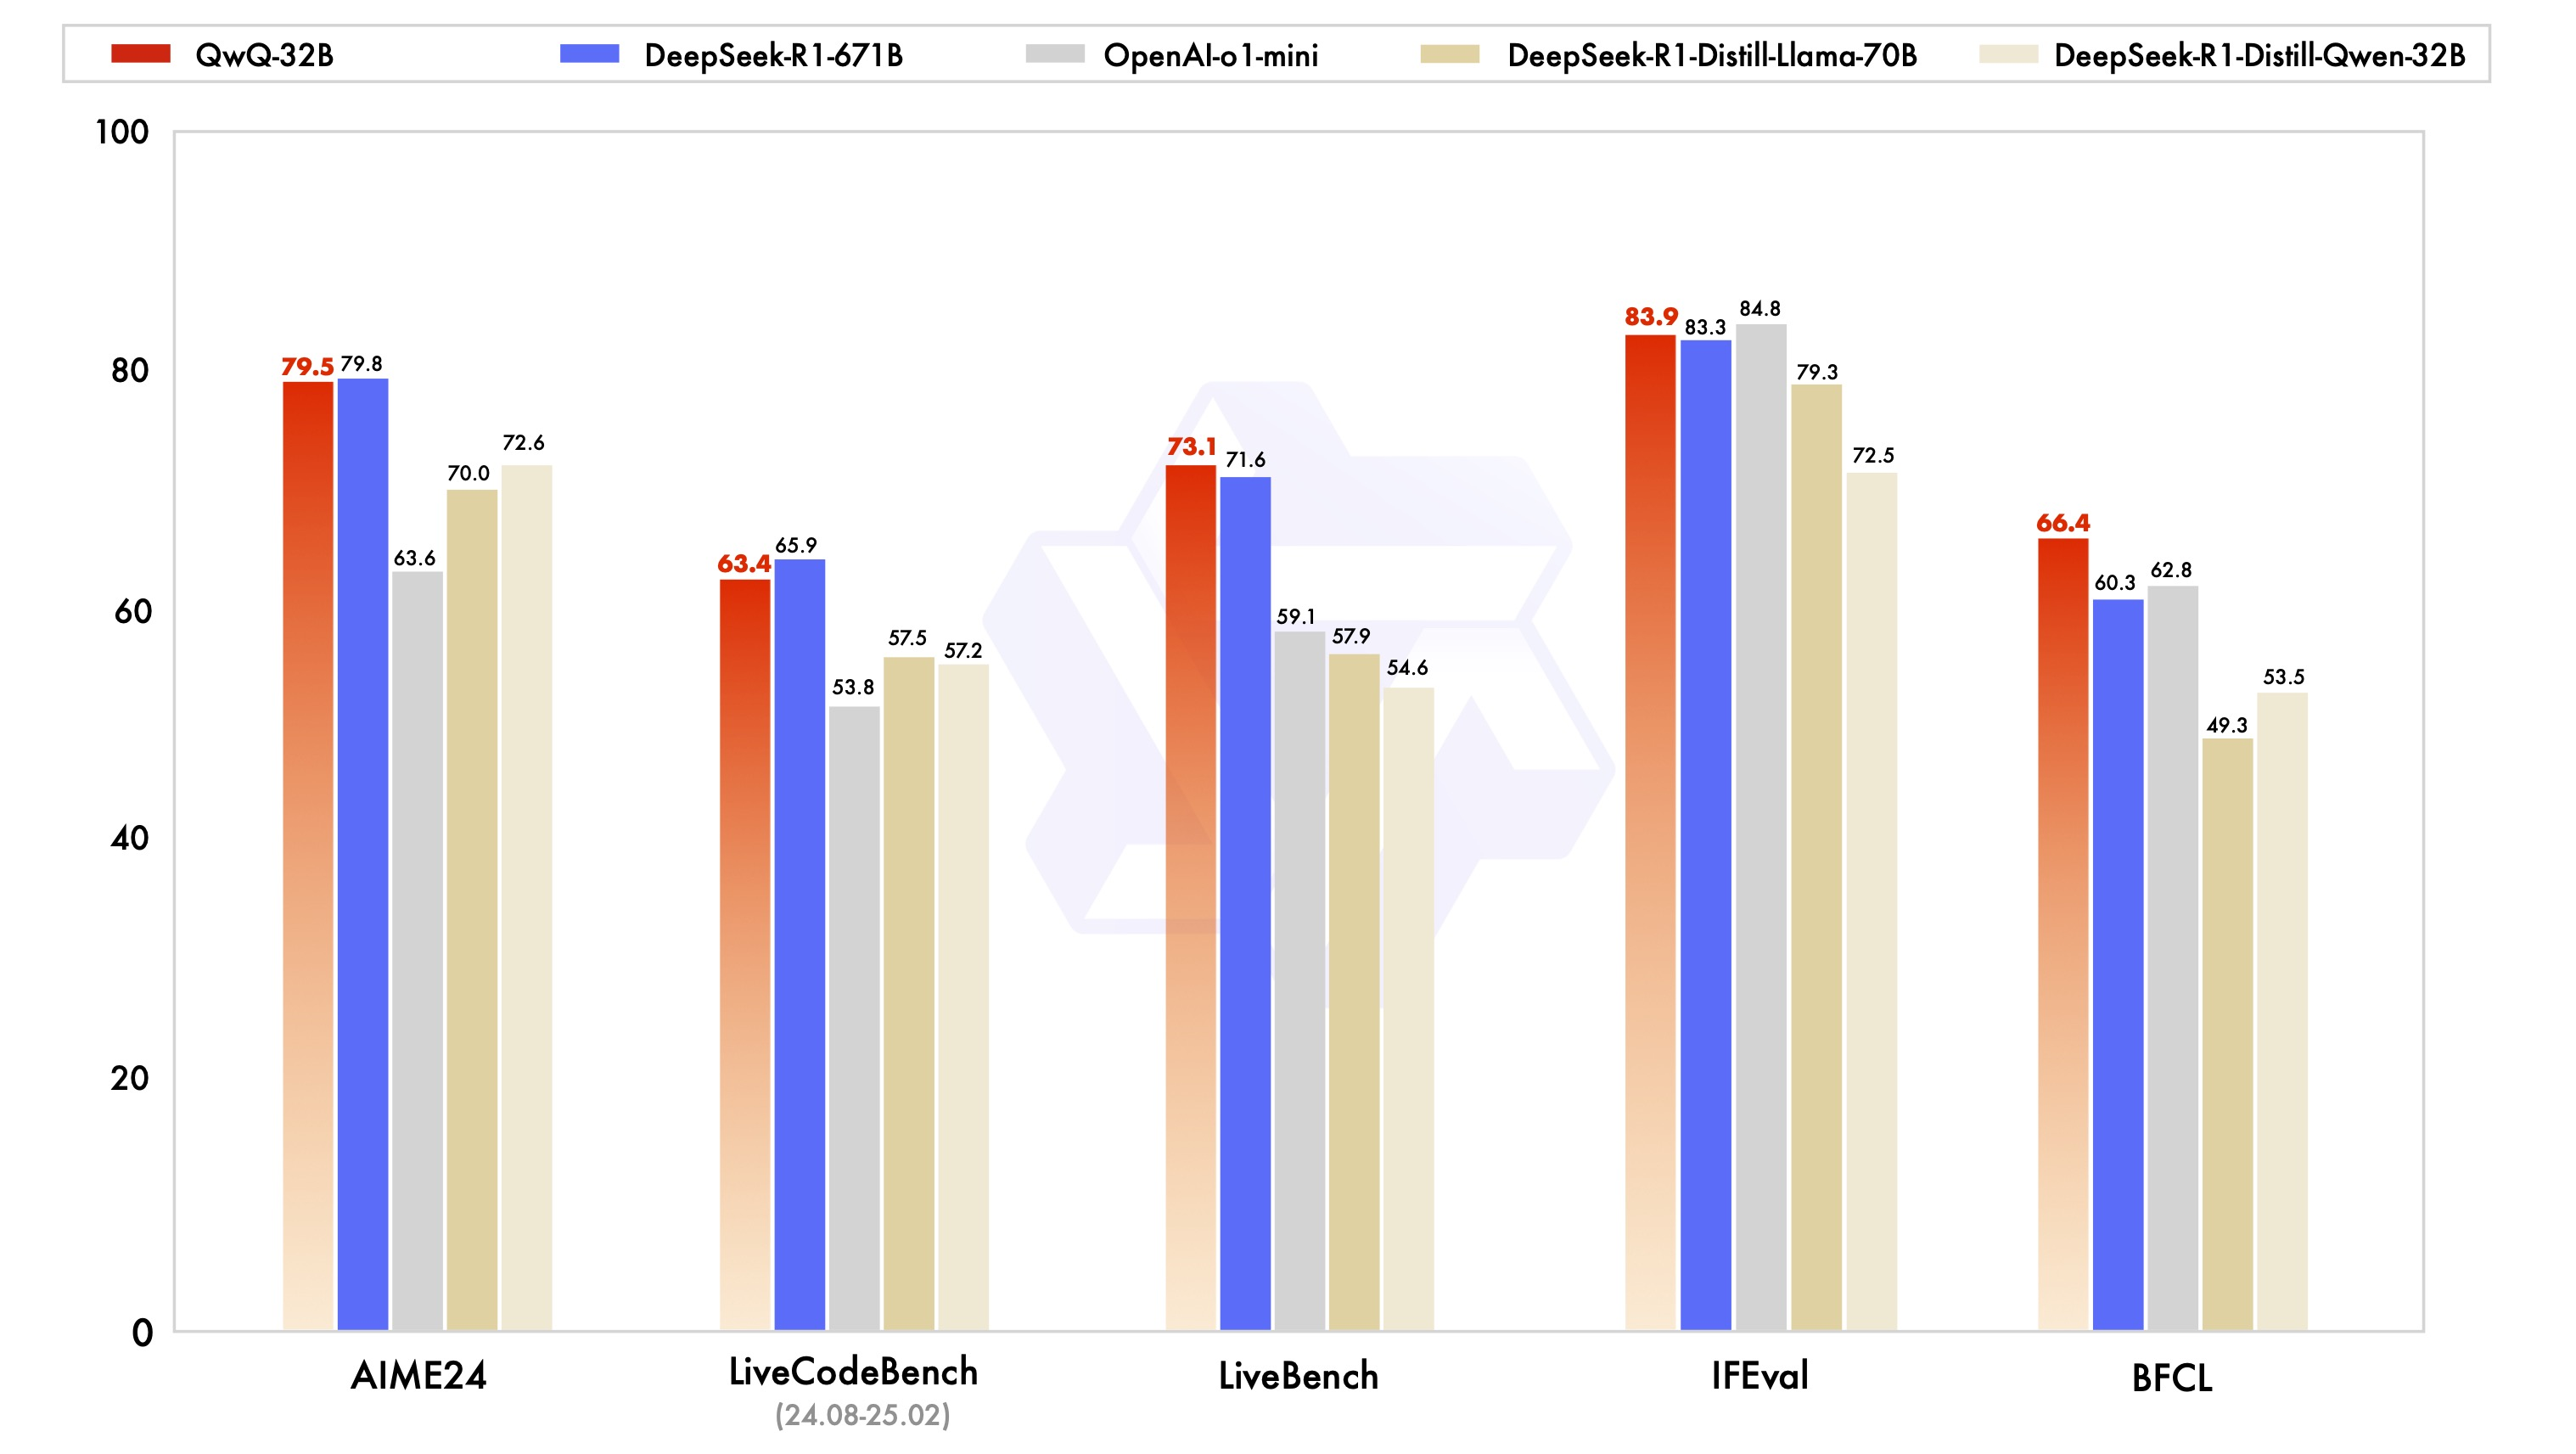
\includegraphics[width=1\linewidth]{figure/qwq-32b-final.jpg}
    \caption{QwQ performance in benchmarks}
    \label{fig:qwq-performance}
\end{figure}

\paragraph{}\autocite{chen_parallel_2025} is a paper exploring a new way of improving \acrshort{llm} performance through a new kind of scaling rule. Rather than using parameter scaling (making larger dense or MoE models), or inference time scaling (reasoning models), this instead uses one set of parameters being executed in parallel and the results combined together. By creating a model using this method, they were able to come up with something that requires a fraction of the memory than a similar performing dense model while having improved lantecy. Table \ref{tab:compare} is a copy of the table from this paper showing the advantages and disadvantages of different LLM scaling methods.

%Table from study
{
\begin{table}[t]
\caption{Copy of comparison table from \textcite{chen_parallel_2025}}
\centering
\resizebox{\linewidth}{!}{
\begin{tabular}{lllll}
\toprule
Method & Inference Time & Inference Space & Training Cost & Specialized Strategy \\
\midrule
Dense Scaling &  \emoji{figure/neutral_face} Moderate & \emoji{figure/rage} High & \emoji{figure/rage} Pre-training only & \emoji{figure/grin} No \\
MoE Scaling & \emoji{figure/grin} Low & \emoji{figure/rage} High & \emoji{figure/rage} Pre-training only & \emoji{figure/rage} \makecell[l]{Load balancing} \\
\makecell[l]{Inference-Time Scaling} & \emoji{figure/rage} High & \emoji{figure/neutral_face} Moderate & \emoji{figure/grin} \makecell[l]{Post-training} & \emoji{figure/rage} \makecell[l]{RL / reward data} \\
Parallel Scaling & \emoji{figure/neutral_face} Moderate & \emoji{figure/neutral_face} Moderate & \emoji{figure/grin} \makecell[l]{Pre- or Post-training} & \emoji{figure/grin} No \\
\bottomrule
\end{tabular}
}
\label{tab:compare}
\end{table}
}

\subsection{Image generation models}
\paragraph{}

\subsection{Fine Tuning models}

\subsection{\acrfull{rag}}
\acrshort{rag} is a technique that allows an LLM to access external data. This is done by having the LLM send the data to another model. This is converted to an embedding/vector. The embedding model uses this to search through a index of a knowledge base. This index also contains vectors that are compared against the vectors of the query. The retrieved information if then sent back to the LLM to generate a response. \acrshort{rag} could be used in a variety of applications including helping lawyers, doctors, and financial analysts with questions. \autocite{merritt_what_2025}.

\subsection{Agentic \acrshort{ai}}
\paragraph{}Agentic \acrshort{ai} is capable of goal-oriented, autonomous action and is adaptable. These \acrshort{ai}s are based on generative \acrshort{ai} such as LLMs. Unlike conventional LLMs they are not limited to the information they are trained on as they can do things such as independently gather new information. Like an LLM an agentic \acrshort{ai} can be interacted with through a natural language prompt, making them simpler to use than other software products. \autocite{noauthor_what_2025}.

\paragraph{}According to \textcite{pounds_what_2024} agentic \acrshort{ai} uses a four step process:
\begin{enumerate}
    \item Perceive
    \item Reason
    \item Act
    \item Learn
\end{enumerate}

\paragraph{}The last step called learn involves gathering data from the system in use, and using it to train future iterations of the model. This creates a feedback loop called the data flywheel.

\subsection{\acrshort{ai} in Scenario Generation}

\paragraph{}

\subsection{Character \acrshort{ai} and chatbots}

\chapter{Aims and Objectives}
\subsubsection*{Aims:}
Use AI to improve realism, immersion, and to assist learning

\subsubsection{Objectives:}
\begin{enumerate}
    \item Investigate how \acrshort{ai} models can interact with students during cyber security training scenarios
    \begin{itemize}
        \item Setup and test chatbots acting as employees and thread actors in challenges
        \item Test the ability of \acrshort{llm}s to give hints and tips without giving away complete answers
    \end{itemize}
    \item Investigate the use of AI models to generate scenarios for use in Cyber Security training simulations
    \begin{itemize}
        \item Determine if \acrshort{llm}s are suitable for generating malware for students to analyze
        \item Demonstrate using LLMs to generate narrative content for scenarios in an automated fashion
    \end{itemize}
\end{enumerate}

\chapter{Studies}
\section{Study 1 - Hackerbot}
\subsection{Description}

\paragraph{}Hackerbot is a program that is used as part of Hacktivity and SecGen to play the role of an attacker or an examiner. It's code is included as part of the SecGen repository on GitHub. It works by interacting with students over an \acrfull{irc} server hosted in a virtual machine alongside hackerbot. They can then access hackerbot through an \acrshort{irc} client such as Pidgin through one of more \acrshort{VM}s that are part of an educational cybersecurity scenario environment such as a \acrshort{ctf}, cyberrange, or lab exercise. When prompted as part of a challenge is can then execute commands inside the \acrfull{VM} it is installed within to attack other \acrshort{VM}s in the training environment or to perform actions remotely. It is pre-programmed by SecGen during the creation and configuration of it's host \acrlong{VM} with a scenario file including all the challenges, prompt, and commands it will need for that specific exercise.

\paragraph{}Currently hackerbot are quite limited. It responds to specific commands, and any other input that does not fall within those is passed to a simple chatbot called \acrfull{alice}. \acrshort{alice} is an older generation technology that uses pre-determined responses when given a question. It does not use any form of \acrlong{dl} or \acrfull{ann}. The primary aim of this study is to make hackerbot more realistic. One of the ways of doing this is to get hackerbot to respond in a more human like manner to inputs outside of it's hard-coded commands by using \acrshort{llm} instead of \acrshort{alice}. Using more advanced chatbots may also allow for replacing of commands that need to be strictly typed and spelled to a more natural interface - though this would require the use of more advanced techniques such as agentic AI. It could also allow hackerbot to take on the role of specific characters that are 

\backmatter


\printglossary[type=\acronymtype]
\printbibliography{}
\section*{Use of \acrshort{ai}}
\paragraph{}Aside from \acrshort{ai} models descibred in experiments, AI based grammer assistance was used in the making of this document through a system called Writeful that's part of the Overleaf LaTeX suite.



\printglossary


\end{document}
